\section{Nonuniformity of the Decision Tree Model}
\label{tree:sorting:nonuniformity}

A nonuniform model of computation is a model where inputs of different lengths
can be processed by different algorithms. In contrast with models equivalent to
the Universal Turing Machine, where one algorithm can solve a problem on inputs
of any size, in a nonuniform model one can have one algorithm per possible size
of the input.

In our model, an algorithm is a decision tree. Since the size and shape of
this tree depends on the size of the input, we have to conclude that the
decision tree model is nonuniform.

\begin{figure}
\center
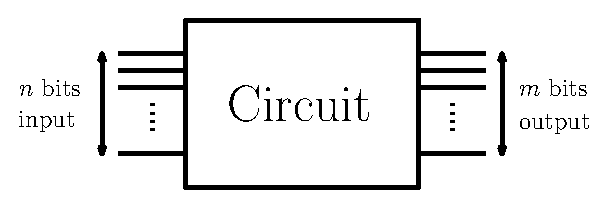
\includegraphics[height=0.15\textheight]{fig/sorting/model/circuit}
\caption{A Boolean circuit with \(n\) bits of input and \(m\) bits of output.}
\label{fig:sorting:nonuniformity:circuit}
\end{figure}

Another example of such a model is circuit complexity. A Boolean circuit,
see \ref{fig:sorting:nonuniformity:circuit}, can be seen as an algorithm with
fixed size input and fixed size output. Since we want to solve problems of any
size, to each computational problem we assign a family of Boolean circuits
\(C_1,C_2,\ldots,C_n,\ldots\) that solve instances of the problem for every
possible input size. We say that this circuit family is P-uniform if there
exists a Turing machine running in time polynomial in \(n\) for which \(n\) is
the input and \(C_n\) is the output.

For all the problems we study, one can make the parallel between the
complexity analysis on the number of comparisons required to solve them and an
analysis of their complexity in the Boolean circuit model. The goal of the
next two paragraphs is to illustrate this equivalence.

As a general fact, we can design an algorithm for any problem in the decision
tree model with fixed input size \(n\) and fixed output set \(\Gamma\) using
the following approach. We generate the finite set containing all possible
decision trees with \(\card{\Gamma}\) leaves. To each node of the trees we
generated corresponds a query of the form \(q(x_1,\ldots,x_n)\) where
\(x_1,\ldots,x_n\) is the input vector. We must assign queries to the nodes
in a way that is consistent with the assignment on the leaves. Moreover, a
query must allow us to distinguish between at least one leaf and a nonempty
set of other remaining possible outputs. Otherwise this query would have only
one children and would be pointless. Note that all of this can be computed
without an input. At each node we simply simulate both ``yes'' and ``no''
answers without bothering the oracle and generate the left and right subtrees
according to which answer corresponds to which subtree. Since there are
finitely many such decision trees, we can generate them all and keep the one
with minimum height \(h\). To solve an instance of size \(n\) we can walk
through the decision tree we built, branching according to the answers we get
from the oracle.

This is equivalent to building \(C_n\), a circuit of depth \(h\). For problems
where \(h\) is polynomial in \(n\), for each problem size we have a circuit
\(C_n\) giving the correct output in polynomial time. Unfortunately, there
exist such problems for which constructing \(C_n\) takes time exponential
in \(n\). Hence, the circuit families for those problems are not P-uniform. As
a last remark, note that the complexity class consisting of problems for which
\(h\) is at most polynomial in \(n\) while constructing \(C_n\) is at most
exponential in \(n\) is called P/poly.

